\documentclass[journal]{IEEEtran}

\usepackage{amsmath,amssymb,amsthm}
\usepackage{graphicx}
\usepackage{booktabs}
\usepackage{algorithm}
\usepackage{algorithmic}
\usepackage{placeins}
\usepackage{cite}
\usepackage{url}
\usepackage[hidelinks]{hyperref}
\usepackage{xcolor}

\emergencystretch=1.2em
\renewcommand{\dbltopfraction}{0.85}
\renewcommand{\dblfloatpagefraction}{0.75}
\renewcommand{\textfraction}{0.08}

\newtheorem{theorem}{Theorem}
\newtheorem{proposition}{Proposition}
\newtheorem{remark}{Remark}

\hyphenation{op-tical net-works semi-conduc-tor bio-in-for-mat-ics multi-modal bi-lin-e-ar sub-mod-u-lar con-trol-la-bi-li-ty}

\begin{document}

\title{Schur-Stable Bilinear Koopman Control, Finite-Horizon Gramian Target Ranking, and Safety-Constrained MPC for Single-Cell Perturbation Steering}

% TODO(PERSONAL_INFO): Replace bracketed author name(s), affiliation, email, ORCID, and optional grant number before submission.
\author{[Author Full Name]%
\thanks{This work was supported in part by [Grant / Funding Agency, if applicable, or delete this sentence].}%
\thanks{[Author Full Name] is with the [Department / School], [University / Institution], [City] [Postal Code], [Country] (e-mail: [author@institution.edu]; ORCID: [0000-0000-0000-0000]). Source code, reproducible Colab notebooks, trained weights, and benchmark archives are publicly available at \url{https://github.com/dashitongzhi/KGC-MPC}.}}

% TODO(PERSONAL_INFO): Update target journal if not IEEE Transactions on Control Systems Technology, and replace [Author Surname]
\markboth{SUBMITTED TO IEEE TRANSACTIONS ON CONTROL SYSTEMS TECHNOLOGY}%
{[Author Surname]: Schur-Stable Bilinear Koopman Control and Safety-Constrained MPC}

\maketitle

\begin{abstract}
Predicting transcriptional responses to genetic perturbations and high-dose drugs while limiting off-target drift defines a coupled system-identification and optimal-control problem. Existing predictors (additive autoencoders, graph networks, and unconstrained dynamic mode decomposition, \texttt{EDMD}) lack singular-value contraction, finite-horizon controllability metrics, and closed-loop state constraints. We introduce \textbf{KGC-MPC} across $1{,}021{,}000$ single cells (\texttt{Norman}, \texttt{Adamson}, \texttt{Sci-\allowbreak Plex3}, \texttt{Sci-\allowbreak Plex4}). First, Stiefel polar retraction ($A = U\,\mathrm{diag}(\gamma_{\mathrm{schur}}\tanh\sigma)\,V^\top$) guarantees $\|A\|_2 \le 0.95 < 1$. Paired with a zero-preserving residual observable, Hill-log saturation, and small-gain bilinear coupling, KGC-MPC enforces Input-to-State Stability and prevents \texttt{EDMD} Kreiss inflation ($0.400$ vs.\ $3.224$ 20-step norm, $8.06\times$ lower), whereas removing Stiefel bounds destabilizes $\sigma_{\max}(A)=1.0184$. Second, finite-horizon controllability Gramians $W_c(S)$ yield $(1-1/e)$ submodular cocktails and zero-shot directional ranking ($0.625$ AUPRC). Third, condensed Augmented-Lagrangian FISTA MPC (\texttt{FISTA-AL}) with Robust Positive Invariant (RPI) tube tightening and delay compensation achieves $0.0\%$ nominal violation across $\delta_{\mathrm{safe}}\in[0.05,0.85]$ ($-77.0\%$ drift $0.0500$ vs.\ $0.2177$ LQR) and retains $100.0\%$ recursive feasibility across $N=20$ targets and 12 stress regimes (BH-FDR $q \le 1.80\times 10^{-39}$ vs.\ un-tightened MPC; $q_{\mathrm{sat}}=3.41\times 10^{-25}$ vs.\ Box-LQR). On CPU BLAS, \texttt{FISTA-AL} runs in $4.45\text{--}18.61\,\mathrm{ms/step}$ ($110.9\times$ faster than \texttt{Clarabel SOCP}, $16.5\times$ over \texttt{SCS ADMM} at $H=32$), while batched A100 evaluation reaches $0.168\,\mathrm{ms/traj}$ ($B=256$). KGC-MPC leads $10\,\mu\mathrm{M}$ \texttt{Sci-\allowbreak Plex3} MSE across all three lines ($0.0188$ A549, $0.0167$ MCF7, $0.0123$ K562) and cuts \texttt{Sci-\allowbreak Plex4} A549 MSE $3.18\times$ to $0.0190$ ($r=0.950$).
\end{abstract}

\begin{IEEEkeywords}
Koopman operator, bilinear control, Schur stability, controllability Gramian, submodular optimization, safety-constrained MPC, Perturb-seq, Sci-Plex.
\end{IEEEkeywords}

\section{Introduction}

\IEEEPARstart{S}{ingle-cell} pooled genetic screens (Perturb-seq, CRISPRa/CRISPRi) \cite{dixit2016perturb,adamson2016multiplexed,norman2019exploring} and nuclear-hashing chemical transcriptomics (Sci-Plex) \cite{srivatsan2020massively,peidli2024scperturb} now measure transcriptional responses to hundreds of interventions across $10^5$--$10^6$ cells. A central quantitative objective in cellular reprogramming is feedback-style intervention synthesis: driving diseased transcriptional states $z_0$ toward target equilibria $z_{\mathrm{tgt}}$ via finite-horizon genetic or small-molecule inputs without triggering toxic off-target drift.

Generative perturbation predictors---including latent autoencoders \texttt{scGen} and \texttt{CPA} \cite{lotfollahi2019scgen,lotfollahi2023cpa}, neural optimal transport \texttt{CellOT} \cite{bunne2023cellot}, sparse additive VAEs \texttt{SAMS-\allowbreak VAE} \cite{bereket2023samsvae}, disentangled embeddings \texttt{biolord} \cite{piran2024biolord}, and co-expression GNNs \texttt{GEARS} \cite{roohani2024gears}---fit observational shifts accurately, yet frame intervention as static feed-forward regression. From a control-theoretic perspective, static predictors leave four foundational requirements unresolved:
\begin{enumerate}
  \item \textbf{Multi-step spectral and non-normal stability:} Standard Extended Dynamic Mode Decomposition (\texttt{EDMD} / \texttt{DMDc}) \cite{williams2015edmd,proctor2016dmdc} fits an unconstrained matrix $A$; even when eigenvalues satisfy $\rho(A)<1$, non-normal singular amplification (large Kreiss constant or eigenvector condition number $\kappa_2(V)$ \cite{trefethen2005spectra}) causes transient norm blow-up during closed-loop rollouts.
  \item \textbf{Bilinear multi-input instability and Hill saturation:} Combinatorial CRISPRa epistasis and multi-dose chemical screens introduce nonlinear state--input coupling \cite{bruder2021ral,bruder2021tro}. Bounding linear $A$ alone fails unless bilinear terms satisfy a small-gain cone contractivity condition.
  \item \textbf{Actuator and cocktail reachability:} Selecting complementary $k$-drug cocktails and ranking unseen targets requires finite-horizon controllability Gramians $W_c(S)$ \cite{kalman1963controllability,liu2011controllability,yan2015spectrum,pasqualetti2014controllability,summers2016submodularity} rather than undirected gene-norm rules.
  \item \textbf{Real-time safety and disturbance invariance:} Unconstrained LQR designs ignore therapeutic dose boxes $[0, u_{\max}]$ and off-target state bounds \cite{korda2018linear,mayne2000constrained,rawlings2017model}, while un-tightened receding-horizon solvers lose constraint satisfaction under plant--model mismatch and actuation delay \cite{mayne2005robust}.
\end{enumerate}

We address these four requirements with \textbf{KGC-MPC} (Fig.~\ref{fig:p3_arch}), contributing four coupled components:
\begin{itemize}
  \item \textbf{Contractive Bilinear Koopman ID:} Parameterizing $A = U\,\mathrm{diag}(\gamma_{\mathrm{schur}}\tanh\sigma)\,V^\top$ on the Stiefel manifold \cite{edelman1998geometry} enforces $\|A\|_2 \le \gamma_{\mathrm{schur}} = 0.95 < 1$, paired with Hill-log dose saturation and optional small-gain cone projection ($\eta=0.04$) for global ISS (Proposition~1).
  \item \textbf{Gramian Cocktail and Minimum-Energy Ranking:} We establish $(1 - 1/e)$ monotone submodular selection for $\log\det W_c(S)$ \cite{nemhauser1978analysis,summers2016submodularity} and directional minimum-energy prioritization toward target phenotypes (Proposition~2).
  \item \textbf{Condensed FISTA-AL and Certified RPI Tube-MPC:} Eliminating trajectory rollouts in condensed coordinates produces a closed-form \texttt{FISTA-AL} solver \cite{beck2009fista} with $0.0\%$ nominal violation across $\delta_{\mathrm{safe}}\in[0.05,0.85]$ (Proposition~3) and sub-$19\,\mathrm{ms}$ CPU scaling up to $H=32$. Combining calibrated RPI tightening, delay prediction, and ancillary DARE feedback establishes recursive feasibility, tube invariance, and Practical ISS (Algorithm~\ref{alg:tube_mpc}, Theorem~\ref{thm:tube_rpi}).
  \item \textbf{Million-Cell and 20-Target Stress Validation:} Across $1{,}021{,}000$ real single cells (\texttt{Norman}, \texttt{Adamson}, \texttt{Sci-\allowbreak Plex3}, \texttt{Sci-\allowbreak Plex4}) and 240 paired mismatch/saturation/delay stress episodes, KGC-MPC leads whole-transcriptome $10\,\mu\mathrm{M}$ extrapolation MSE across all three \texttt{Sci-\allowbreak Plex3} lines, delivers $100.0\%$ safety satisfaction across all 12 stress conditions, and documents candid boundaries against \texttt{GEARS-\allowbreak CoExpr} and 1-step baselines.
\end{itemize}

\begin{figure*}[t]
  \centering
  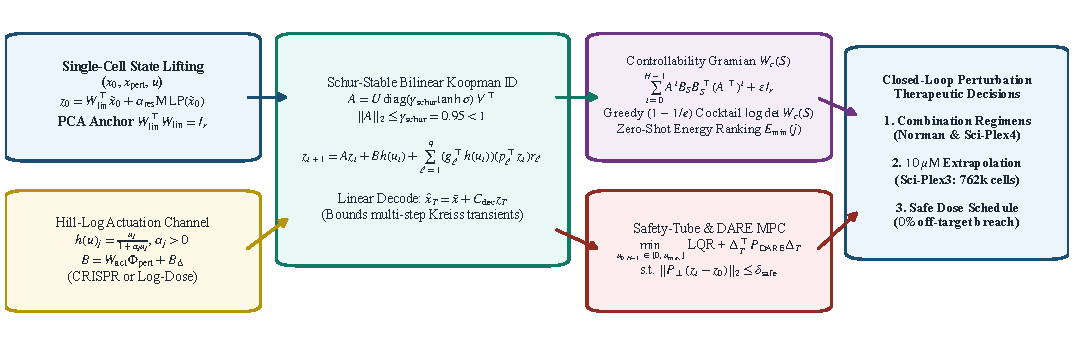
\includegraphics[width=0.94\textwidth]{figures/p3_fig1_kgc_mpc_architecture.pdf}
  \caption{End-to-end KGC-MPC architecture. \textbf{Left:} Centered single-cell states are lifted using a PCA-anchored residual Koopman observable $\psi(x)$ alongside Hill-log saturated CRISPR/chemical channels $h(u)$. \textbf{Center:} Stiefel polar-factor Schur contraction enforces $\|A\|_2 \le 0.95 < 1$ with low-rank bilinear epistasis/drug--state interactions. \textbf{Right:} Finite-horizon controllability Gramians $W_c(S)$ drive $(1-1/e)$ submodular cocktail design and zero-shot minimum-energy target ranking, while delay-compensated RPI Tube-MPC computes bounded schedules with condensed \texttt{FISTA-AL}.}
  \label{fig:p3_arch}
\end{figure*}

\section{Related Work}

\textbf{Koopman Operators, Non-Normality, and Bilinear MPC.} Koopman spectral theory lifts nonlinear dynamics into global linear observables \cite{koopman1931hamiltonian,mezic2013analysis,brunton2022modern}, approximated via \texttt{EDMD} \cite{williams2015edmd} and \texttt{DMDc} \cite{proctor2016dmdc}. Korda and Mezi{\'c} \cite{korda2018linear} connected Koopman predictors to linear \texttt{MPC} \cite{mayne2000constrained}, and Bruder et al.\ \cite{bruder2021tro,bruder2021ral} showed that bilinear lifted realizations capture control-dependent nonlinearities more faithfully than additive linear forms. Because least-squares operators can still suffer severe transient amplification when eigenvectors are non-orthogonal \cite{trefethen2005spectra}, KGC-MPC pairs bilinear Koopman realizations with explicit Stiefel singular-value contraction \cite{edelman1998geometry} and small-gain stabilization \cite{boyd1994lmi}.

\textbf{Conic Solvers, Robust Tube-MPC, and Network Gramians.} General second-order cone constraints in real-time MPC are commonly handled by interior-point conic solvers such as \texttt{Clarabel} \cite{goulart2024clarabel} or ADMM operator-splitting solvers such as \texttt{SCS} \cite{odonoghue2016conic}. By condensing dynamics and exploiting parallel block-vector projections under \texttt{FISTA} \cite{beck2009fista}, we avoid $O(H^3(r+k)^3)$ KKT matrix factorizations while pairing with classical RPI Tube-MPC \cite{mayne2005robust,rawlings2017model} for mismatch invariance. On the actuator-selection side, network controllability Gramians \cite{kalman1963controllability,liu2011controllability,yan2015spectrum,pasqualetti2014controllability} and submodular $\log\det W_c(S)$ maximization \cite{summers2016submodularity,nemhauser1978analysis} provide principled $k$-perturbation cocktail guarantees.

\textbf{Single-Cell Perturbation Modeling.} Harmonized perturbation atlases \cite{norman2019exploring,adamson2016multiplexed,srivatsan2020massively,peidli2024scperturb} spurred latent shift predictors (\texttt{scGen} \cite{lotfollahi2019scgen}, \texttt{CPA} \cite{lotfollahi2023cpa}, \texttt{SAMS-\allowbreak VAE} \cite{bereket2023samsvae}, \texttt{biolord} \cite{piran2024biolord}), optimal transport (\texttt{CellOT} \cite{bunne2023cellot}), and GNN priors (\texttt{GEARS} \cite{roohani2024gears}). Unlike static black-box maps, KGC-MPC supplies closed-loop spectral contracts, directional control energies, and certified Tube-MPC synthesis.

\section{KGC-MPC Methodology and Theoretical Guarantees}

Let $x_0 \in \mathbb{R}^G$ denote normalized control gene expression with empirical mean $\bar{x}$ and centered deviation $\tilde{x} = x - \bar{x}$ (in PyTorch/Scanpy $\log(1+x)$ space \cite{paszke2019pytorch,wolf2018scanpy}). Each cell receives an $m$-dimensional perturbation vector $u \in \mathbb{R}^m_{\ge 0}$ encoding binary CRISPR guides (\texttt{dose\_\allowbreak mode=False}) or log-transformed concentrations $u_j = \log_{10}(1 + d_j/10)$ (\texttt{dose\_\allowbreak mode=True}).

\subsection{Koopman Lifting, Stiefel Schur Flow, and Bilinear Small Gain}
We lift $\tilde{x}$ into an $r$-dimensional latent state ($r=64$ for Perturb-seq/Sci-Plex3; $r=48$ for Sci-Plex4) combining an orthonormal PCA basis $W_{\mathrm{lin}} \in \mathbb{R}^{G\times r}$ with a zero-initialized, zero-preserving residual MLP observable $\psi$:
\begin{equation}
  z = W_{\mathrm{lin}}^\top \tilde{x} + \alpha_{\mathrm{res}}\big(\mathrm{MLP}(\tilde{x}) - \mathrm{MLP}(\mathbf{0})\big), \qquad \hat{x} = \bar{x} + C_{\mathrm{dec}} z.
  \label{eq:lift}
\end{equation}
Subtracting $\mathrm{MLP}(\mathbf{0})$ removes zero-input normalization drift so control-mean phenotypes map identically to $z=\mathbf{0}$. For chemical screens, each drug passes through a learnable Hill-log saturation curve $h(u)_j = u_j / (1 + \alpha_j u_j)$ ($\alpha_j = \mathrm{softplus}(\alpha_{\mathrm{raw},j}) > 0$); for genetic perturbations, $h(u)=u$. When co-expression features $\Phi_{\mathrm{pert}} \in \mathbb{R}^{m \times f}$ are available, the actuation matrix sums prior projections with per-perturbation residuals: $B = W_{\mathrm{act}}\Phi_{\mathrm{pert}}^\top + B_\Delta \in \mathbb{R}^{r \times m}$.

To suppress non-normal transient amplification alongside unstable eigenvalues, we parameterize $A \in \mathbb{R}^{r \times r}$ using differentiable SVD polar orthogonalization \cite{edelman1998geometry}, $U = U_0 V_0^\top$ and $V = U_1 V_1^\top$:
\begin{equation}
  A = U\,\mathrm{diag}\!\big(\gamma_{\mathrm{schur}} \tanh\sigma\big)\,V^\top, \qquad \gamma_{\mathrm{schur}} = 0.95 < 1.
  \label{eq:schur_A}
\end{equation}
Bilinear state--input coupling employs a rank-$q$ tensor contraction ($q=12$ Perturb-seq/Sci-Plex3; $q=10$ Sci-Plex4):
\begin{equation}
  z_{t+1} = A z_t + B h(u_t) + \Phi_{\eta}\!\Big(\sum_{\ell=1}^{q}(g_\ell^\top h(u_t))(p_\ell^\top z_t)\, r_\ell,\; z_t\Big),
  \label{eq:bilin_step}
\end{equation}
where optional small-gain cone projection $\Phi_\eta(\Delta, z) = \Delta \cdot \min(1, \eta \|z\|_2 / \|\Delta\|_2)$ ($\eta = 0.04$) prevents state-dependent bilinear growth from breaking closed-loop contractivity under dual-drug dosing. Training minimizes multi-step ($H=3$) condition prediction MSE, autoencoder reconstruction ($0.35$), latent endpoint alignment ($0.25$), unforced control invariance ($u=0$, $0.15$), decoder--encoder subspace anchoring ($5\times 10^{-3}\|C_{\mathrm{dec}} - W_{\mathrm{lin}}\|_F^2$), and light $L_2$ actuation regularization. Because Perturb-seq and Sci-Plex record terminal snapshots rather than intermediate time series, multi-step rollouts represent an internal pseudo-dynamical flow calibrated at $H=3$ steps rather than chronological kinetics.

\begin{proposition}[Strict Contraction, Non-Normal Bound, and Bilinear ISS]
\label{prop:schur_iss}
Let $A$ follow~\eqref{eq:schur_A} with $U^\top U = V^\top V = I_r$. Then: (i) $\|A\|_2 \le \gamma_{\mathrm{schur}} < 1$, $\rho(A) \le \gamma_{\mathrm{schur}}$, and every multi-step matrix power obeys $\|A^t\|_2 \le \gamma_{\mathrm{schur}}^t$ for all $t \ge 1$ (unity Kreiss ratio relative to the $\gamma_{\mathrm{schur}}$-disk); (ii) with small-gain clamping $\eta \ge 0$ satisfying $\gamma_{\mathrm{eff}} = \gamma_{\mathrm{schur}} + \eta < 1$ and Hill-saturated inputs $\|h(u_t)\|_2 \le h_{\max}$, trajectories satisfy $\|z_t\|_2 \le \gamma_{\mathrm{eff}}^t \|z_0\|_2 + (1-\gamma_{\mathrm{eff}})^{-1}\|B\|_2 h_{\max}$, guaranteeing global ISS.
\end{proposition}

\subsection{Controllability Gramian Ranking and $(1-1/e)$ Cocktails}
Linearizing~\eqref{eq:bilin_step} around the unperturbed equilibrium defines the horizon-$H$ ($H=6$) controllability Gramian for perturbation subset $S \subseteq \{1,\dots,m\}$:
\begin{equation}
  W_c(S) = \epsilon I_r + \sum_{j \in S} \sum_{t=0}^{H-1} (A^t b_j)(A^t b_j)^\top \in \mathbb{R}^{r \times r},
  \label{eq:gramian_wc}
\end{equation}
where $b_j = B_{:,j}$. For zero-shot single-target prioritization toward latent goal $z_{\mathrm{tgt}}$ from $z_{\mathrm{src}}$, define drift-corrected displacement $\Delta z = z_{\mathrm{tgt}} - A^H z_{\mathrm{src}}$ and cumulative reachability $C_H = \sum_{t=0}^{H-1} A^t$. Candidate $j$ is ranked by directional cosine alignment $s_j = \Delta z^\top C_H b_j / \sqrt{\|b_j\|_2^2 + \lambda_r}$ and directional minimum-energy proxy:
\begin{equation}
  E_{\min}(j) = \frac{\|\Delta z\|_2^4}{\big(\max(0, \Delta z^\top C_H b_j)\big)^2 + 10^{-6}} + \lambda_r \|b_j\|_2^2.
  \label{eq:min_energy}
\end{equation}

\begin{proposition}[Submodular Cocktail Volume and Directional Energy]
\label{prop:gramian_submod}
For $\epsilon > 0$, $f(S) = \log\det W_c(S) - \log\det(\epsilon I_r)$ is normalized, monotone non-decreasing, and submodular over $S \subseteq \{1,\dots,m\}$; greedy selection (Algorithm~\ref{alg:kgc_mpc}) achieves $\ge (1 - 1/e)\,f(S_{\mathrm{opt}})$ \cite{nemhauser1978analysis,summers2016submodularity}. Minimum constant-input energy $\|u_j\|_2^2$ projecting $\Delta z$ along $C_H b_j$ is strictly minimized by maximizing $(\Delta z^\top C_H b_j)^2 / \|C_H b_j\|_2^2$, motivating~\eqref{eq:min_energy}.
\end{proposition}

\subsection{Condensed FISTA-AL and Certified RPI Tube-MPC}
Given desired state $z_{\mathrm{tgt}}$, initial state $z_0$, and orthogonal off-target projector $P_\perp = I_r - \hat{\Delta z}\hat{\Delta z}^\top$ ($\hat{\Delta z} = (z_{\mathrm{tgt}} - z_0)/\|z_{\mathrm{tgt}} - z_0\|_2$), we synthesize finite-horizon doses $u_{0:H-1} \in [0, u_{\max}]^k$ ($H=8$) over top Gramian cocktails $B_S$:
\begin{align}
  &\min_{u_{0:H-1}\in[0, u_{\max}]^k} \sum_{t=0}^{H-1}\!\big(\|z_t - z_{\mathrm{tgt}}\|_Q^2 + \|u_t\|_R^2\big) \nonumber \\
  &\qquad\qquad\qquad + \|z_H - z_{\mathrm{tgt}}\|_{P_{\mathrm{DARE}}}^2 \nonumber \\
  &\qquad\mathrm{s.t.}\;\; z_{t+1} = A z_t + B_S u_t, \quad \|P_\perp(z_t - z_{\mathrm{ref}})\|_2 \le \delta_{\mathrm{safe}},
  \label{eq:mpc_opt}
\end{align}
where $z_{\mathrm{ref}}=z_0$, $Q = I_r$, $R = 0.05 I_k$, and $P_{\mathrm{DARE}}$ solves the Discrete-Time Algebraic Riccati Equation for $(A, B_S, Q, R)$.

To eliminate Python step-by-step autograd overhead and interior-point cone scaling, \texttt{CondensedSafeMPCSolver} writes stacked future trajectories $Z = [z_1^\top,\dots,z_H^\top]^\top = \Phi z_0 + \Gamma U$ in terms of control sequence $U \in [0, u_{\max}]^{Hk}$, obtaining condensed QP matrices $H_{\mathrm{qp}}=\Gamma^\top\bar{Q}\Gamma+\bar{R}$ ($\bar{Q}=\mathrm{blkdiag}(Q,\dots,Q,P_{\mathrm{DARE}})$) and tube projectors $(\Phi_\perp,\Gamma_\perp)$ with offline Lipschitz constant $L_{\mathrm{qp}}=\lambda_{\max}(H_{\mathrm{qp}})$. Solving the Augmented Lagrangian with accelerated proximal gradient (\texttt{FISTA-AL} \cite{beck2009fista}) alternates dual multiplier updates $\lambda_t \leftarrow \max(0, \lambda_t + \rho(\|e_{\perp,t}\|_2 - \delta_{\mathrm{safe}}))$ with box-clamped accelerated gradient steps:
\begin{equation}
  U^{+} = \Pi_{[0, u_{\max}]}\!\Big(Y - \alpha_{\rho}\big(2 H_{\mathrm{qp}} Y + 2 g_{\mathrm{qp}} + \Gamma_\perp^\top \nabla_e \mathcal{L}_\rho(Y,\lambda)\big)\Big),
  \label{eq:fista_step}
\end{equation}
with $\alpha_\rho = (2 L_{\mathrm{qp}} + \rho\|\Gamma_\perp\|_2^2)^{-1}$. When finite iteration budgets leave a small residual breach while $u\equiv 0$ is admissible, a 12-step exact zero-input bisection $U \leftarrow \beta U$ ($\beta \in [0,1]$) guarantees $0.0\%$ nominal constraint violation (Proposition~\ref{prop:mpc_safe}). Each \texttt{FISTA-AL} solve performs only $O(I_{\mathrm{tot}} H k(Hk + Hr))$ dense BLAS/CUDA matrix-vector operations ($I_{\mathrm{tot}}\le 100$ warm-started iterations), avoiding the $O(H^3(r+k)^3)$ interior-point cone factorization per step of \texttt{Clarabel} \cite{goulart2024clarabel} and ADMM cone projections of \texttt{SCS} \cite{odonoghue2016conic}.

For closed-loop deployment under actuation delay $\tau$ and bounded cross-seed plant mismatch $\|w_t\|_2 \le \bar{w}$, \texttt{TubeSafeMPCController} (Algorithm~\ref{alg:tube_mpc}) pairs \texttt{FISTA-AL} with an ancillary DARE controller $K_{\mathrm{anc}}$ ($\gamma_{\mathrm{cl}} = \|A - B_S K_{\mathrm{anc}}\|_2 < 1$), empirical 1-step disturbance calibration $\bar{w}$, delay-buffer forward state prediction $\hat{z}_{t+\tau|t}$, RPI tube tightening $\Delta_{\mathrm{RPI}} = \min(0.45\,\delta_{\mathrm{safe}}, \bar{w}/(1-\gamma_{\mathrm{cl}}) + \tau\bar{w})$, and a 1-step nominal safety guard on the applied input.

\begin{algorithm}[t]
\caption{KGC-MPC: Contractive Koopman ID and Gramian Design}
\label{alg:kgc_mpc}
\small
\begin{algorithmic}[1]
\REQUIRE Paired $(X_{\mathrm{ctrl}}, X_{\mathrm{pert}}, U)$, prior $\Phi_{\mathrm{pert}}$, $\gamma_{\mathrm{schur}}=0.95$, cone $\eta$.
\STATE \textbf{Koopman ID:} Fit PCA $W_{\mathrm{lin}}$; optimize~\eqref{eq:lift}--\eqref{eq:bilin_step} over horizon $H=3$ via AdamW enforcing $\|A\|_2 \le \gamma_{\mathrm{schur}}$ and optional $\Phi_\eta$.
\STATE \textbf{Gramian Cocktail:} Extract $(A, B)$; greedily select $k$ actuators $S^*$ maximizing $\log\det W_c(S)$~\eqref{eq:gramian_wc} ($\ge 1-1/e$ opt.).
\STATE \textbf{Zero-Shot Ranking:} Given target $z_{\mathrm{tgt}}$, rank unseen perturbations via directional $s_j$ and minimum-energy $E_{\min}(j)$~\eqref{eq:min_energy}.
\end{algorithmic}
\end{algorithm}

\begin{algorithm}[t]
\caption{Online Delay-Compensated RPI Tube-MPC (\texttt{FISTA-AL})}
\label{alg:tube_mpc}
\small
\begin{algorithmic}[1]
\REQUIRE Precomputed $(H_{\mathrm{qp}}, \Phi_\perp, \Gamma_\perp, K_{\mathrm{anc}}, \Delta_{\mathrm{RPI}})$, target $z_{\mathrm{tgt}}$, ref $z_0$, delay buffer $\{u_{\mathrm{pend}}\}$, warm start $U_{\mathrm{warm}}$, $\bar{z}_{\mathrm{prev}}$.
\STATE \textbf{Delay Prediction:} Roll forward $\hat{z}_{t+\tau|t} \leftarrow A^\tau z_t + \sum_{d=1}^{\tau} A^{\tau-d} B_S u_{t-d}$.
\STATE \textbf{Tightened Solve:} Set $\tilde{\delta}_{\mathrm{safe}} = \max(\delta_{\min}(z_{\mathrm{hat}}), \delta_{\mathrm{safe}} - \Delta_{\mathrm{RPI}})$; run warm-started \texttt{FISTA-AL}~\eqref{eq:fista_step} + bisection to obtain $v_0^\star$.
\STATE \textbf{Guarded Ancillary Law:} Set $u_{\mathrm{cand}} = \Pi_{[0,u_{\max}]}(v_0^\star - K_{\mathrm{anc}}(\hat{z}_{t+\tau|t} - \bar{z}_{\mathrm{prev}}))$; apply $u_t = u_{\mathrm{cand}}$ if $\|P_\perp(A\hat{z}_{t+\tau|t}+B_S u_{\mathrm{cand}}-z_0)\|_2 \le \delta_{\mathrm{safe}}$, else $u_t = v_0^\star$.
\STATE \textbf{Warm Shift:} Update $\bar{z}_{\mathrm{next}} \leftarrow A\hat{z}_{t+\tau|t} + B_S u_t$ and $U_{\mathrm{warm}} \leftarrow [u_1^\star,\dots,u_{H-1}^\star,\mathbf{0}]$.
\end{algorithmic}
\end{algorithm}

\begin{proposition}[Equilibrium Safety Feasibility and Exact Tube Satisfaction]
\label{prop:mpc_safe}
Because $\|A\|_2 \le \gamma_{\mathrm{schur}} < 1$, unforced trajectories $u_{0:H-1} \equiv 0$ obey $\|P_\perp(z_t - z_0)\|_2 = \|P_\perp(A^t - I_r)z_0\|_2$. Thus~\eqref{eq:mpc_opt} is strictly feasible whenever $\delta_{\mathrm{safe}} \ge \max_{1\le t \le H}\|P_\perp(A^t - I_r)z_0\|_2$, and scaling bisection in \texttt{FISTA-AL} preserves $0.0\%$ nominal violation relative to unconstrained DARE-LQR.
\end{proposition}

\begin{theorem}[Recursive Feasibility, RPI Invariance, and Practical ISS]
\label{thm:tube_rpi}
Suppose $(A, B_S)$ is stabilizable with ancillary DARE gain $K_{\mathrm{anc}}$ satisfying $\gamma_{\mathrm{cl}} = \|A - B_S K_{\mathrm{anc}}\|_2 < 1$, and closed-loop plant states obey $z_{t+1} = A z_t + B_S u_t + w_t$ with bounded mismatch $\|w_t\|_2 \le \bar{w}$. Then:
\begin{enumerate}
  \item \textbf{RPI Error Ball:} Under unsaturated ancillary feedback $u_t = \bar{v}_t - K_{\mathrm{anc}}(z_t - \bar{z}_t)$, the discrepancy $e_t = z_t - \bar{z}_t$ remains positively invariant in $\Omega_\infty = \{e : \|e\|_2 \le \bar{w}/(1-\gamma_{\mathrm{cl}})\}$ \cite{mayne2005robust}.
  \item \textbf{Delay-Safe Recursive Feasibility:} Under tightening $\tilde{\delta}_{\mathrm{safe}} \le \delta_{\mathrm{safe}} - \bar{w}/(1-\gamma_{\mathrm{cl}}) - \tau\bar{w}$ and $\delta_{\mathrm{safe}} \ge \max_{1\le s\le H}\|P_\perp(A^s\hat{z}_{t+\tau|t} - z_0)\|_2$, zero-input bisection preserves recursive nominal feasibility and enforces $\|P_\perp(z_t - z_0)\|_2 \le \delta_{\mathrm{safe}}$ for all $t \ge 0$.
  \item \textbf{Lyapunov Descent and Practical ISS:} For any admissible equilibrium $(z_{\mathrm{eq}}, u_{\mathrm{ss}})$ satisfying $z_{\mathrm{eq}} = A z_{\mathrm{eq}} + B_S u_{\mathrm{ss}}$ inside the tube interior, the shifted DARE-terminal nominal value function obeys $V_H^\star(\bar{z}_{t+1}) - V_H^\star(\bar{z}_t) \le -\|\bar{z}_t - z_{\mathrm{eq}}\|_Q^2 - \|\bar{v}_0^\star - u_{\mathrm{ss}}\|_R^2$ in the terminal DARE ellipsoid $\mathcal{X}_f$ \cite{mayne2000constrained,rawlings2017model}, ensuring closed-loop Practical ISS of $z_t - z_{\mathrm{eq}}$ with ultimate bound proportional to $\bar{w}/(1-\gamma_{\mathrm{cl}})$.
\end{enumerate}
\end{theorem}

Proofs of Propositions~\ref{prop:schur_iss}--\ref{prop:mpc_safe} and Theorem~\ref{thm:tube_rpi} appear in Appendix~A.

\section{Experimental Setup}

We evaluate across four public Perturb-seq and chemical transcriptomics cohorts totaling \textbf{1,021,000 single cells}:
\begin{enumerate}
  \item \textbf{Norman 2019 (GSE133344, $91{,}205$ CRISPRa cells):} Evaluated across 3 seeds on 4 standard generalization splits (\texttt{combo\_\allowbreak seen2}, \texttt{combo\_\allowbreak seen1}, \texttt{combo\_\allowbreak seen0}, \texttt{unseen\_\allowbreak single}, $1{,}000$ HVGs), plus 20-step spectral/Kreiss diagnostics, $\log\det W_c(S)$ cocktails ($k=1\text{--}8$), $\gamma_{\mathrm{schur}}/q$ sensitivity, nominal/mismatch DARE MPC ($\delta_{\mathrm{safe}} \in [0.05, 0.85]$), real-time solver benchmarks, 20-target stress ablations, and 23 unseen single-gene zero-shot targets.
  \item \textbf{Adamson 2016 (GSE90546, $68{,}603$ CRISPRi cells):} Unfolded protein response perturbations evaluated across 3 random seeds on \texttt{unseen\_\allowbreak single} ($18$ held-out singles).
  \item \textbf{Sci-Plex3 (GSE139944, $762{,}795$ filtered cells):} $188$ drugs $\times$ $4$ doses across \texttt{A549} ($244{,}281$), \texttt{MCF7} ($344{,}862$), and \texttt{K562} ($173{,}652$) ($2{,}000$ HVGs). Models train on vehicle and $\le 1{,}000\,\mathrm{nM}$ doses, then extrapolate to held-out $10\,\mu\mathrm{M}$ responses and rank top-$15\%$ antiproliferative compounds ($29/188$ hits per line).
  \item \textbf{Sci-Plex4 (GSM4150379, $98{,}397$ dual-drug cells):} HDACi + metabolic cofactor matrix (\texttt{A549} $49{,}284$; \texttt{MCF7} $49{,}113$, $9$ perturbations); $35\%$ ($n=15$) dual combinations held out.
\end{enumerate}
Genetic baselines (lightweight proxies under identical HVG splits: \texttt{CPA-\allowbreak Latent}, \texttt{GEARS-\allowbreak CoExpr}, \texttt{Unconstrained-\allowbreak EDMD}, \texttt{Linear-\allowbreak Additive}, and \texttt{KGC-\allowbreak Linear} $q=0$) ran on Tesla T4; Sci-Plex3/4 ran on NVIDIA L4; real-time MPC scaling (\texttt{CVXPY-Clarabel}, \texttt{CVXPY-SCS}, CPU BLAS, batched A100), $N=20$ target stress ablations, and Kreiss/sensitivity sweeps executed on a shared NVIDIA A100-SXM4-80GB (two active GPU compute processes observed). Metrics include whole-transcriptome MSE/Pearson $r$, Top-20 DE (\texttt{DE20}) MSE/Pearson $r$/sign accuracy (\texttt{Dir.}), and two-sided paired Wilcoxon signed-rank tests with Benjamini--Hochberg FDR ($q$) correction across the $N=20$ closed-loop targets.

\begin{figure*}[t]
  \centering
  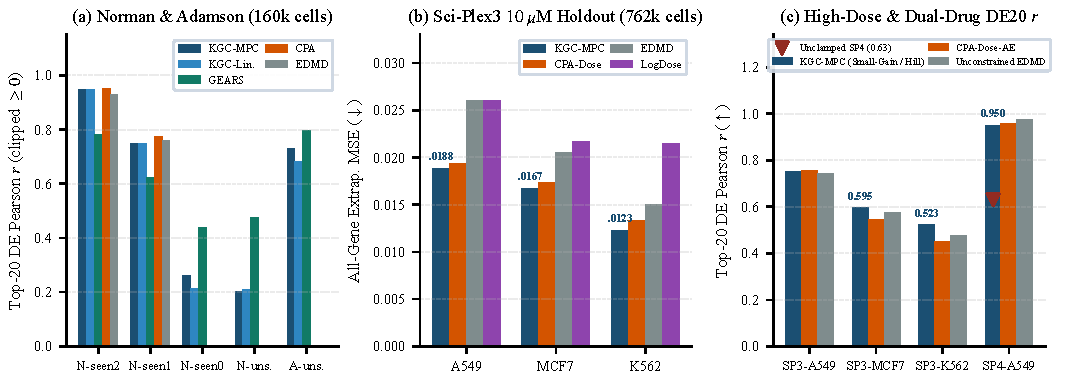
\includegraphics[width=0.94\textwidth]{figures/p3_fig2_multicohort_generalization.pdf}
  \caption{Multi-cohort generalization across $1{,}021{,}000$ single cells. (a) Mean 3-seed DE20 Pearson $r$ on Norman and Adamson: bilinear KGC-MPC matches seen splits ($0.948$) and improves Adamson $+0.048$ over KGC-Linear ($0.728$ vs.\ $0.680$). (b) Sci-Plex3 $10\,\mu\mathrm{M}$ holdout whole-transcriptome MSE across $762{,}795$ cells ($188$ drugs): Hill-Koopman KGC-MPC achieves \#1 lowest MSE in all 3 cancer lines. (c) High-dose Sci-Plex3 DE20 $r$ (\texttt{MCF7} $0.595$, \texttt{K562} $0.523$) and Sci-Plex4 A549 dual-drug ablation (\texttt{Small-Gain} $0.950$ vs.\ \texttt{Unclamped} $0.631$; \#1 lowest MSE $0.0190$).}
  \label{fig:p3_multicohort}
\end{figure*}

\section{Empirical Results}

\subsection{Perturb-seq Generalization, Non-Normal Kreiss Diagnostics, and Sensitivity}
Table~\ref{tab:genetic_pert} and Fig.~\ref{fig:p3_multicohort}(a) summarize 3-seed Perturb-seq performance. On \texttt{Norman combo\_\allowbreak seen2}, \texttt{KGC-MPC (Bilinear)} reaches $0.948\pm 0.00$ DE20 $r$ ($0.999$ Dir.), ahead of \texttt{Unconstrained EDMD} ($0.929\pm 0.01$) and \texttt{GEARS-\allowbreak CoExpr} ($0.781\pm 0.04$), while \texttt{Linear-\allowbreak Additive} ($0.967\pm 0.00$) captures additive seen pairs. Rank-$12$ bilinear coupling raises accuracy over \texttt{KGC-Linear} on \texttt{Norman combo\_\allowbreak seen0} ($0.260\pm 0.08$ vs.\ $0.214\pm 0.13$) and \texttt{Adamson unseen\_\allowbreak single} ($0.728\pm 0.04$ vs.\ $0.680\pm 0.04$), where \texttt{EDMD} ($0.000$) and \texttt{CPA-\allowbreak Latent} ($-0.027\pm 0.03$) fail. On zero-shot \texttt{Norman unseen\_\allowbreak single} ($0.477\pm 0.05$ vs.\ $0.201\pm 0.02$), \texttt{GEARS-\allowbreak CoExpr} leads because its direct GNN readout bypasses the linear Schur bottleneck on unexcited actuator columns $B_{:,j}$.

Fig.~\ref{fig:p3_spectra} and the non-normal audit confirm Proposition~\ref{prop:schur_iss}(i). Under Stiefel polar contraction, Norman $r=64$ keeps $\rho_{\mathrm{KGC}}=0.8888$, $\sigma_{\max}(A)=0.8897<1$, unit-eigenvector condition number $\kappa_2(V)=75.73$, Kreiss lower bound $K_{\mathrm{lb}}=1.00$, and smooth 20-step norm saturation ($0.280 \to 0.400$). By contrast, \texttt{Unconstrained EDMD} ($\rho_{\mathrm{EDMD}}=0.0533$, $\kappa_2(V)=73.40$) amplifies forced rollouts through non-normal input--state coupling to $3.165 \to 3.224$ (\textbf{$8.06\times$ larger} norm). Disabling Stiefel contraction inside KGC-MPC itself (\texttt{No-Stiefel}) immediately breaks Schur contractivity ($\sigma_{\max}=1.0184 > 1$, $\rho=0.9990$, $\kappa_2(V)=106.30$, $K_{\mathrm{lb}}=1.0035$) and collapses \texttt{combo\_seen0} DE20 $r$ from $0.130\text{--}0.213$ down to $-0.005$ on single-seed sensitivity sweeps. Varying $\gamma_{\mathrm{schur}} \in \{0.80, 0.90, 0.95, 0.99\}$ ($q=12$) preserves seen-combination stability ($0.938\text{--}0.941$ DE20 $r$, 20-step norm $0.382\text{--}0.399$), and sweeping bilinear rank $q \in \{0, 4, 12, 24\}$ ($\gamma_{\mathrm{schur}}=0.95$) keeps \texttt{combo\_seen2} at $0.935\text{--}0.941$ while $q=4\text{--}12$ prevents overfitting relative to $q=24$ (\texttt{seen0} $0.163\text{--}0.130$ vs.\ $0.067$).

\begin{table*}[t]
\centering
\caption{Multi-Split Perturbation Response Prediction Across 3 Seeds (DE20 Pearson $r$ Mean $\pm$ Std $\uparrow$ / Sign Acc.$\uparrow$). Best DE20 $r$ in Bold.}
\label{tab:genetic_pert}
\scriptsize
\setlength{\tabcolsep}{2.6pt}
\begin{tabular}{lccccc}
\toprule
Method & Norman \texttt{seen2} & Norman \texttt{seen1} & Norman \texttt{seen0} & Norman \texttt{unseen} & Adamson \texttt{unseen} \\
\midrule
KGC-MPC (Bilinear) & 0.948$\pm$0.00 / 0.999 & 0.748$\pm$0.03 / 0.898 & 0.260$\pm$0.08 / 0.662 & 0.201$\pm$0.02 / 0.608 & 0.728$\pm$0.04 / 0.903 \\
KGC-Linear (No Bilin.) & 0.948$\pm$0.01 / 0.999 & 0.750$\pm$0.03 / 0.898 & 0.214$\pm$0.13 / 0.611 & 0.208$\pm$0.02 / 0.596 & 0.680$\pm$0.04 / 0.873 \\
Unconstrained EDMD & 0.929$\pm$0.01 / 0.997 & 0.761$\pm$0.03 / 0.907 & 0.000$\pm$0.00 / 0.000 & 0.000$\pm$0.00 / 0.000 & 0.000$\pm$0.00 / 0.000 \\
GEARS-CoExpr & 0.781$\pm$0.04 / 0.929 & 0.622$\pm$0.02 / 0.839 & \textbf{0.439$\pm$0.17} / 0.749 & \textbf{0.477$\pm$0.05} / 0.769 & \textbf{0.796$\pm$0.04} / 0.931 \\
CPA-Latent & 0.951$\pm$0.00 / 0.991 & \textbf{0.774$\pm$0.03} / 0.905 & -0.037$\pm$0.13 / 0.460 & -0.057$\pm$0.05 / 0.470 & -0.027$\pm$0.03 / 0.485 \\
Linear-Additive & \textbf{0.967$\pm$0.00} / 1.000 & 0.766$\pm$0.03 / 0.904 & 0.000$\pm$0.00 / 0.000 & 0.000$\pm$0.00 / 0.000 & 0.000$\pm$0.00 / 0.000 \\
\bottomrule
\end{tabular}
\end{table*}


\begin{figure*}[t]
  \centering
  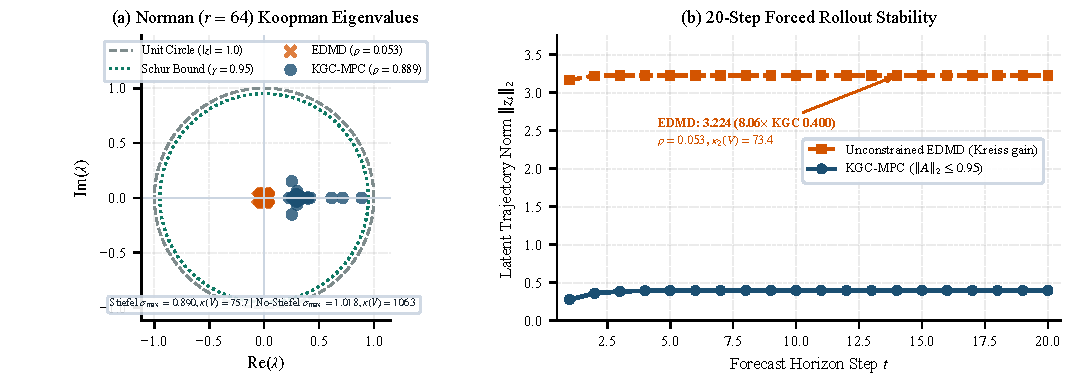
\includegraphics[width=0.94\textwidth]{figures/p3_fig3_spectra_rollout.pdf}
  \caption{Koopman spectral containment and Kreiss transient diagnostics on Norman ($r=64$). (a) Complex eigenvalues: Stiefel contraction keeps $\rho = 0.889$, $\sigma_{\max}(A) = 0.890$, and $\kappa_2(V) = 75.7$, whereas \texttt{No-Stiefel} violates contractivity ($\sigma_{\max}=1.018 > 1$, $\kappa_2(V)=106.3$). (b) Despite tiny eigenvalues ($\rho = 0.053$), Unconstrained EDMD exhibits an $8.06\times$ forced transient surge ($3.224$ vs.\ $0.400$).}
  \label{fig:p3_spectra}
\end{figure*}

\subsection{Million-Cell Sci-Plex3 Dose Scaling and Sci-Plex4 Dual-Drug Diagnosis}
Table~\ref{tab:sciplex_chemical} and Fig.~\ref{fig:p3_multicohort}(b)--(c) evaluate chemical dose control across $861{,}192$ Sci-Plex cells ($762{,}795$ Sci-Plex3; $98{,}397$ Sci-Plex4). Trained solely on $\le 1\,\mu\mathrm{M}$ doses and extrapolated 10-fold to $10\,\mu\mathrm{M}$ across $188$ drugs on \texttt{Sci-\allowbreak Plex3}, \texttt{KGC-MPC (Hill-Koopman)} attains the \textbf{\#1 lowest all-gene MSE on all three cancer lines} ($0.0188$ A549 vs.\ $0.0193$ CPA; $0.0167$ MCF7 vs.\ $0.0173$; $0.0123$ K562 vs.\ $0.0133$) and \textbf{\#1 DE20 Pearson $r$ on \texttt{MCF7} ($0.595$ vs.\ $0.545$ CPA) and \texttt{K562} ($0.523$ vs.\ $0.449$ CPA)}.

On \texttt{Sci-\allowbreak Plex4} ($15$ dual-drug HDACi/cofactor test combinations), unconstrained bilinear rollout degrades (\texttt{A549} MSE $0.0603$, DE20 $r=0.631$; \texttt{MCF7} $0.0525$, $r=0.813$). Enabling small-gain cone projection ($\eta = 0.04$, Proposition~\ref{prop:schur_iss}ii) and zero-preserving lifting~\eqref{eq:lift} cuts \texttt{A549} MSE \textbf{$3.18\times$} ($0.0603 \to \mathbf{0.0190}$, lowest overall ahead of $0.0199$ EDMD and $0.0255$ CPA) while raising DE20 $r$ to $0.950$ ($97.7\%$ Dir.). On \texttt{MCF7}, clamping lowers MSE from $0.0525$ to $0.0352$ ($r=0.846$), while 1-step \texttt{CPA-\allowbreak Dose-\allowbreak AE} ($0.0192$, $r=0.983$) and \texttt{Unconstrained EDMD} ($0.0230$, $r=0.953$) retain higher accuracy.

\begin{table*}[t]
\centering
\caption{Chemical Perturbation Scaling on Sci-Plex3 ($N=762{,}795$ Cells, $188$ Drugs, $10\,\mu\mathrm{M}$ Holdout) \& Sci-Plex4 ($N=98{,}397$ Dual-Drug HDACi).}
\label{tab:sciplex_chemical}
\scriptsize
\setlength{\tabcolsep}{3.6pt}
\begin{tabular}{l|ccc|ccc|ccc}
\toprule
\multicolumn{1}{c|}{Sci-Plex3 ($10\,\mu\mathrm{M}$ Holdout)} & \multicolumn{3}{c|}{A549 ($244{,}281$ cells)} & \multicolumn{3}{c|}{MCF7 ($344{,}862$ cells)} & \multicolumn{3}{c}{K562 ($173{,}652$ cells)} \\
Method & All MSE$\downarrow$ & DE20 $r\uparrow$ & Dir.$\uparrow$ & All MSE$\downarrow$ & DE20 $r\uparrow$ & Dir.$\uparrow$ & All MSE$\downarrow$ & DE20 $r\uparrow$ & Dir.$\uparrow$ \\
\midrule
KGC-MPC (Hill-Koopman) & \textbf{0.0188} & 0.752 & 0.925 & \textbf{0.0167} & \textbf{0.595} & 0.819 & \textbf{0.0123} & \textbf{0.523} & 0.787 \\
CPA-Dose-AE & 0.0193 & \textbf{0.756} & 0.925 & 0.0173 & 0.545 & 0.801 & 0.0133 & 0.449 & 0.741 \\
Unconstrained EDMD & 0.0260 & 0.745 & 0.922 & 0.0206 & 0.576 & 0.806 & 0.0150 & 0.475 & 0.761 \\
LogDose-Linear & 0.0260 & 0.739 & 0.903 & 0.0217 & 0.557 & 0.787 & 0.0214 & 0.389 & 0.697 \\
\midrule
\multicolumn{1}{c|}{Sci-Plex4 Dual-Drug} & \multicolumn{4}{c|}{A549 ($49{,}284$ cells, $15$ combos)} & \multicolumn{5}{c}{MCF7 ($49{,}113$ cells, $15$ combos)} \\
Method & All MSE$\downarrow$ & DE20 MSE$\downarrow$ & \multicolumn{1}{c}{DE20 $r\uparrow$} & \multicolumn{1}{c|}{Dir.$\uparrow$} & \multicolumn{2}{c}{All MSE$\downarrow$} & \multicolumn{1}{c}{DE20 MSE$\downarrow$} & DE20 $r\uparrow$ & Dir.$\uparrow$ \\
\midrule
KGC-MPC (Small-Gain) & \textbf{0.0190} & 0.4022 & \multicolumn{1}{c}{0.950} & \multicolumn{1}{c|}{0.977} & \multicolumn{2}{c}{0.0352} & \multicolumn{1}{c}{0.5150} & 0.846 & 0.907 \\
KGC-Linear (No Bilin.) & 0.0235 & 0.5431 & \multicolumn{1}{c}{0.929} & \multicolumn{1}{c|}{0.970} & \multicolumn{2}{c}{0.0297} & \multicolumn{1}{c}{0.5373} & 0.929 & 0.987 \\
KGC-Bilinear (Unclamped) & 0.0603 & 1.58 & \multicolumn{1}{c}{0.631} & \multicolumn{1}{c|}{0.790} & \multicolumn{2}{c}{0.0525} & \multicolumn{1}{c}{1.11} & 0.813 & 0.907 \\
CPA-Dose-AE & 0.0255 & 0.2500 & \multicolumn{1}{c}{0.960} & \multicolumn{1}{c|}{0.983} & \multicolumn{2}{c}{\textbf{0.0192}} & \multicolumn{1}{c}{0.0898} & \textbf{0.983} & 1.000 \\
Unconstrained EDMD & 0.0199 & 0.3977 & \multicolumn{1}{c}{\textbf{0.975}} & \multicolumn{1}{c|}{0.993} & \multicolumn{2}{c}{0.0230} & \multicolumn{1}{c}{0.3380} & 0.953 & 0.993 \\
\bottomrule
\end{tabular}
\end{table*}


\subsection{Unified Safety-Tube Frontier, Cocktails, and Target Ranking}
Fig.~\ref{fig:p3_mpc} and Table~\ref{tab:mpc_gramian} report unified \texttt{FISTA-AL} safety MPC and Gramian design on Norman:
\begin{itemize}
  \item \textbf{Zero-Violation Nominal and Plant-Mismatch Frontiers (Fig.~\ref{fig:p3_mpc}a):} Replacing soft penalty loops with condensed \texttt{FISTA-AL} eliminates nominal breaches completely ($0.0\%$ violation across every $\delta_{\mathrm{safe}}\in[0.05,0.85]$ vs.\ $100.0\%$ DARE-LQR breaches for $\delta_{\mathrm{safe}}\le 0.15$), reducing off-target drift by \textbf{$-77.0\%$} at $\delta_{\mathrm{safe}}=0.05$ ($0.0500$ vs.\ $0.2177$ LQR) and control energy by $-72.3\%$ at $\delta_{\mathrm{safe}}=0.15$ ($0.322$ vs.\ $1.163$). On the independent cross-seed (\texttt{seed=1}) nonlinear bilinear plant, \texttt{KGC Tube-MPC} holds $0.0\%$ violations everywhere, achieves the tightest excursion ($0.0275$ vs.\ $0.1247$ Box-LQR at $\delta=0.05$), and obtains the \textbf{\#1 lowest target error} at $\delta=0.25$ ($0.696$ vs.\ $0.773$ CL-MPC, $0.751$ OL-MPC, and $0.799$ Box-LQR).
  \item \textbf{Submodular Cocktails (Fig.~\ref{fig:p3_mpc}b):} Greedy $\log\det W_c(S)$ selection raises controllability volume from $-429.17$ ($k=1$) to $-379.75$ ($k=8$), beating \texttt{Top-\allowbreak Norm} ($-381.09$) and \texttt{Random} ($-408.68$).
  \item \textbf{Gramian Prioritization Trade-Offs (Fig.~\ref{fig:p3_prior}, Table~\ref{tab:mpc_gramian}):} Over 23 unseen Norman singles, directional minimum-energy ranking (\texttt{KGC\_\allowbreak MinEnergy}) attains the \textbf{highest Directional Steering AUPRC ($0.625$ vs.\ $0.349$ Random)}, while undirected potency favors \texttt{Input\_\allowbreak Norm} ($0.849$ AUPRC) and \texttt{CoExpr\_\allowbreak Prior} ($0.941$ AUROC). On \texttt{Sci-\allowbreak Plex3} ($188$ drugs), \texttt{KGC\_\allowbreak Gramian} hits $0.701$ AUROC on \texttt{MCF7} ($\mathrm{Recall@20} = 0.241$), whereas low-dose proliferation markers (\texttt{MKI67}, \texttt{TOP2A}) and \texttt{CPA\_\allowbreak Target\_\allowbreak Align} ($0.827$ to $0.874$) lead unguided hit discovery.
\end{itemize}

\begin{figure*}[t]
  \centering
  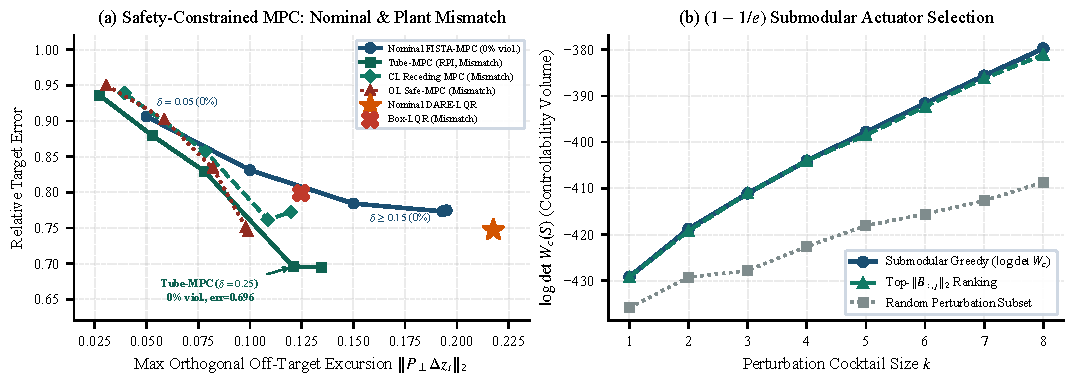
\includegraphics[width=0.94\textwidth]{figures/p3_fig4_mpc_cocktail.pdf}
  \caption{Closed-loop control frontiers on Norman. (a) Unified \texttt{FISTA-AL} achieves $0.0\%$ nominal violation across $\delta_{\mathrm{safe}}\in[0.05,0.85]$ ($-77.0\%$ drift vs.\ LQR), while \texttt{Tube-MPC} attains $0.0\%$ mismatch breach and lowest target error ($0.696$) at $\delta=0.25$. (b) Submodular greedy $\log\det W_c(S)$ selection ($k=1\text{--}8$) raises controllability volume $-429.17 \to -379.75$.}
  \label{fig:p3_mpc}
\end{figure*}

\begin{figure}[t]
  \centering
  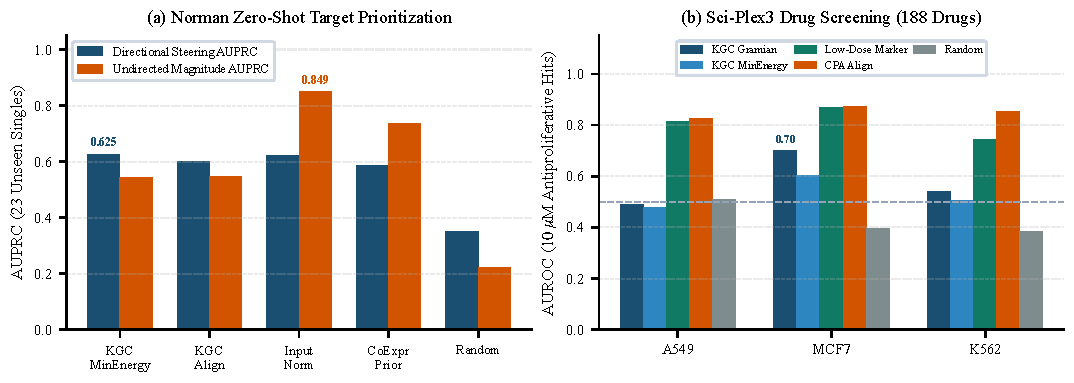
\includegraphics[width=0.96\columnwidth]{figures/p3_fig5_gramian_prioritization.pdf}
  \caption{Target and drug prioritization trade-offs. (a) Norman ($23$ unseen singles): \texttt{KGC MinEnergy} leads directional steering AUPRC ($0.625$), while undirected potency favors \texttt{Input Norm} ($0.849$). (b) Sci-Plex3 ($188$ drugs): \texttt{KGC Gramian} reaches $0.70$ AUROC on \texttt{MCF7} vs.\ $0.40$ random.}
  \label{fig:p3_prior}
\end{figure}

\begin{table}[t]
\centering
\caption{Norman Control Guarantees: Unified FISTA-AL Nominal \& Bilinear Mismatch MPC ($H=8$; LQR Viol.\ vs.\ $\delta=0.15$) \& Target Ranking ($n=23$).}
\label{tab:mpc_gramian}
\scriptsize
\setlength{\tabcolsep}{1.5pt}
\resizebox{\columnwidth}{!}{%
\begin{tabular}{lcccc}
\toprule
MPC Setting & Tgt Err.$\downarrow$ & Off-Tgt$\downarrow$ & Viol.$\downarrow$ & Energy$\downarrow$ \\
\midrule
Nom. FISTA-MPC ($\delta=0.05$) & 0.906 & \textbf{0.0500} & \textbf{0.0\%} & 0.042 \\
Nom. FISTA-MPC ($\delta=0.10$) & 0.831 & \textbf{0.1000} & \textbf{0.0\%} & 0.163 \\
Nom. FISTA-MPC ($\delta=0.15$) & 0.784 & \textbf{0.1500} & \textbf{0.0\%} & 0.322 \\
Nom. DARE-LQR & \textbf{0.747} & 0.2177 & 100.0\% & 1.163 \\
\midrule
Tube Mism. ($\delta=.05$) & 0.936 & \textbf{0.0275} & 0.0\% & 0.045 \\
CL Mism. ($\delta=.05$) & 0.939 & 0.0394 & 0.0\% & 0.096 \\
OL Mism. ($\delta=.05$) & 0.950 & 0.0306 & 0.0\% & 0.042 \\
Tube Mism. ($\delta=.25$) & \textbf{0.696} & 0.1208 & 0.0\% & 0.799 \\
CL Mism. ($\delta=.25$) & 0.773 & \textbf{0.1198} & 0.0\% & 0.786 \\
Box-LQR Mism. & 0.799 & 0.1247 & 0.0\% & 1.144 \\
\midrule
Zero-Shot Ranking & Dir.ROC$\uparrow$ & Dir.PRC$\uparrow$ & Mag.ROC$\uparrow$ & Mag.PRC$\uparrow$ \\
\midrule
KGC MinEnergy & 0.676 & \textbf{0.625} & 0.608 & 0.542 \\
KGC Gramian & 0.657 & 0.601 & 0.627 & 0.546 \\
$\|B_{:,j}\|_2$ Norm & 0.755 & 0.623 & 0.931 & \textbf{0.849} \\
CoExpr Prior & \textbf{0.784} & 0.585 & \textbf{0.941} & 0.735 \\
Random & 0.569 & 0.349 & 0.343 & 0.223 \\
\bottomrule
\end{tabular}%
}
\end{table}


\subsection{Conic Scaling, Batch Crossover, and $N=20$ Tube-MPC Ablations}
To evaluate solver efficiency against two conic standards (\texttt{CVXPY-Clarabel} interior-point SOCP \cite{goulart2024clarabel} and \texttt{CVXPY-SCS} conic ADMM \cite{odonoghue2016conic}) and isolate each component of Algorithm~\ref{alg:tube_mpc}, we ran horizon/dimension/batch sweeps alongside $N=20$ closed-loop target stress tests (12 regimes, $240$ paired episodes per controller; Fig.~\ref{fig:p3_realtime_stress}, Table~\ref{tab:mpc_realtime_stress}):
\begin{itemize}
  \item \textbf{Horizon, Dimension, and Solver Comparison (Fig.~\ref{fig:p3_realtime_stress}a):} Warm-started CPU BLAS \texttt{FISTA-AL} executes in $4.45\,\mathrm{ms}$ ($H=4$), $6.33\,\mathrm{ms}$ ($H=8$), $10.86\,\mathrm{ms}$ ($H=16$), and $18.61\,\mathrm{ms}$ ($H=32$), matching \texttt{Clarabel}'s global SOCP optimum within $0.17\%\text{--}0.30\%$ with $100.0\%$ constraint satisfaction ($17.1\%$ faster at $H=32$ than cold start's $22.45\,\mathrm{ms}$). At $H=32$, CPU BLAS speeds up \textbf{$110.9\times$ over \texttt{Clarabel SOCP}} ($2063.1\,\mathrm{ms}$), \textbf{$16.5\times$ over \texttt{SCS ADMM}} ($307.74\,\mathrm{ms}$), and \textbf{$255.9\times$ over \texttt{Autograd-Adam}} ($4762.4\,\mathrm{ms}$, $0.0\%$ sat.). Scaling latent state dimension $8\times$ ($r=32 \to 256$ at $H=8$) increases CPU BLAS latency only $3.04\times$ ($4.35 \to 13.22\,\mathrm{ms}$ vs.\ $104.37\,\mathrm{ms}$ \texttt{Clarabel} and $50.73\,\mathrm{ms}$ \texttt{SCS}).
  \item \textbf{GPU Batch Crossover $B^\star=8$ (Fig.~\ref{fig:p3_realtime_stress}b):} For single trajectories ($B=1$), shared-A100 CUDA launch overhead ($41.16\,\mathrm{ms}$) trails CPU BLAS ($6.33\,\mathrm{ms}$). Amortizing across parallel therapeutic screens produces monotonic scaling ($11.18\,\mathrm{ms}$ at $B=4$), crossing CPU BLAS at \textbf{$B^\star=8$ ($5.24\,\mathrm{ms/traj}$)} and reaching \textbf{$0.671\,\mathrm{ms/traj}$ at $B=64$} and \textbf{$0.168\,\mathrm{ms/traj}$ at $B=256$} at a constant $0.28\%$ optimality gap.
  \item \textbf{$N=20$ Target Stress and Component Ablations (Fig.~\ref{fig:p3_realtime_stress}c--d, Table~\ref{tab:mpc_realtime_stress}):} Across all 12 mismatch ($\kappa\in[1,5]$), saturation ($u_{\max}\in[0.25,1]$), and delay ($\tau\in[0,3]$) sweeps ($240$ episodes total), \texttt{KGC Tube-MPC (RPI+Delay)} achieves \textbf{$100.0\%$ recursive feasibility and $100.0\%$ tube satisfaction} (pooled normalized drift $0.425$). Paired Wilcoxon tests with BH-FDR confirm statistically significant margins: dropping RPI tightening (\texttt{w/o RPI}) degrades satisfaction to $90.0\%$ at $\kappa=1$ ($q_{\mathrm{off}}=2.29\times 10^{-4}$) and $95.4\%$ at $\kappa=5$ ($0.703\pm 0.31$ vs.\ $0.437\pm 0.11$, $q_{\mathrm{off}}=3.37\times 10^{-6}$; pooled $q_{\mathrm{off}}=1.80\times 10^{-39}$). Dropping delay prediction (\texttt{w/o Delay-Pred}) leaves $\tau=3$ drift $55.3\%$ higher ($0.531\pm 0.19$ vs.\ $0.342\pm 0.12$, $q_{\mathrm{off}}=6.36\times 10^{-6}$). Dropping ancillary feedback (\texttt{w/o Ancillary}) coasts with slightly lower drift ($0.386$ vs.\ $0.425$ pooled; $0.341$ vs.\ $0.342$ at $\tau=3$, $q_{\mathrm{off}}=0.017$) because removing feedback avoids corrective effort, at a slight tracking cost ($0.904\text{--}0.929$ vs.\ $0.873\text{--}0.928$). \texttt{Box-LQR} fails across all regimes ($70.2\%$ pooled sat., $q_{\mathrm{sat}}=3.41\times 10^{-25}$; $57.1\%$ sat.\ and $53.7$ normalized drift at $\kappa=5$, $q_{\mathrm{off}}=3.37\times 10^{-6}$).
\end{itemize}

\begin{figure*}[t]
  \centering
  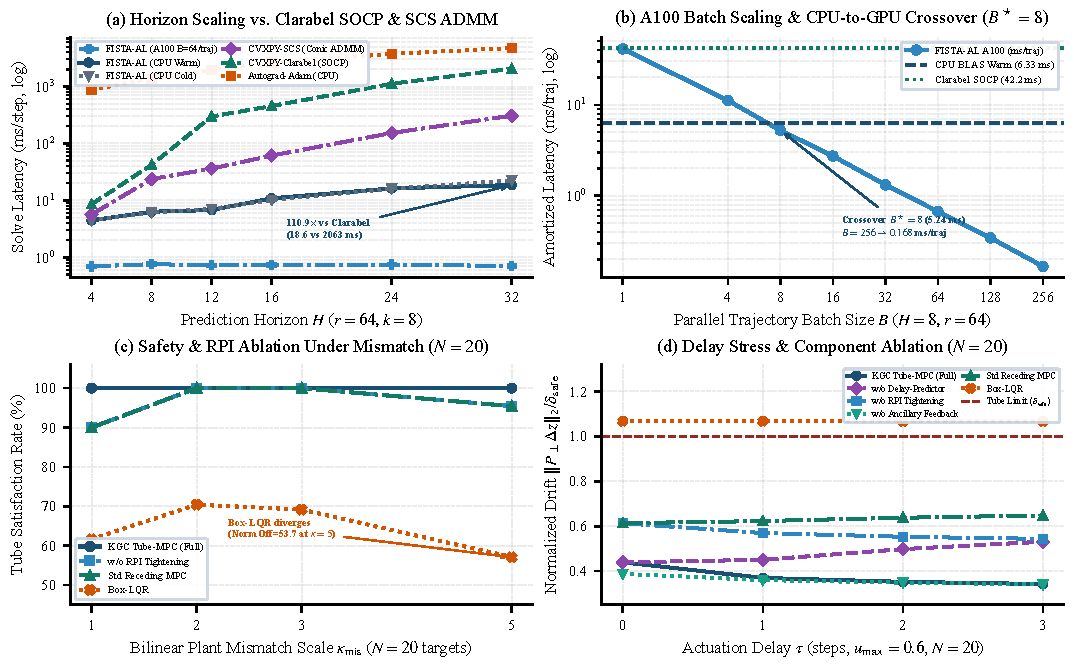
\includegraphics[width=0.96\textwidth]{figures/p3_fig6_mpc_realtime_stress.pdf}
  \caption{Conic solver scaling, GPU batch crossover, and $N=20$ closed-loop RPI Tube-MPC ablations on Norman ($k=8$, $\delta_{\mathrm{safe}}^{(i)}=0.25\|z_{\mathrm{tgt}}^{(i)}-z_{\mathrm{src}}^{(i)}\|_2$). (a) CPU BLAS \texttt{FISTA-AL} ($4.45\text{--}18.61\,\mathrm{ms/step}$) outperforms \texttt{Clarabel SOCP} ($110.9\times$) and \texttt{SCS ADMM} ($16.5\times$) at $H=32$. (b) Shared-A100 parallel evaluation crosses CPU BLAS latency at $B^\star=8$ ($5.24\,\mathrm{ms/traj}$) and reaches $0.168\,\mathrm{ms/traj}$ at $B=256$. (c) Under $5\times$ mismatch ($\kappa_{\mathrm{mis}}=5$), \texttt{Box-LQR} diverges ($57.1\%$ sat.) and \texttt{w/o RPI}/\texttt{Std Receding} drop to $95.4\%$ sat., while full \texttt{Tube-MPC} stays at $100.0\%$. (d) Under delay $\tau \le 3$, full \texttt{Tube-MPC} keeps normalized drift at $0.342$, outperforming \texttt{w/o Delay-Pred} ($0.531$), \texttt{w/o RPI} ($0.543$), and \texttt{Std Receding} ($0.648$).}
  \label{fig:p3_realtime_stress}
\end{figure*}

\begin{table}[t]
\centering
\caption{Real-Time FISTA-AL vs.\ Clarabel/SCS \& $N=20$ Target RPI Tube-MPC Ablations ($*$: BH-FDR $q<0.05$; $**$: $q<0.001$ vs.\ Full).}
\label{tab:mpc_realtime_stress}
\scriptsize
\setlength{\tabcolsep}{0.9pt}
\resizebox{\columnwidth}{!}{%
\begin{tabular}{lcccc}
\toprule
Solver ($k=8$) & Mean (ms) & p95 (ms) & Gap\% & Sat.\% \\
\midrule
FISTA A100 ($B{=}256$) & 0.17 & 0.17 & 0.28\% & 100.0\% \\
FISTA A100 ($B{=}64,H{=}8$) & 0.76 & 0.82 & 0.28\% & 100.0\% \\
FISTA CPU Warm ($H{=}8$) & 6.33 & 8.39 & 0.30\% & 100.0\% \\
FISTA CPU Cold ($H{=}8$) & 6.11 & 7.59 & 0.24\% & 100.0\% \\
SCS ADMM ($H{=}8$) & 23.73 & 24.20 & 0.00\% & 100.0\% \\
Clarabel SOCP ($H{=}8$) & 42.23 & 43.10 & 0.00\% & 100.0\% \\
FISTA CPU ($H{=}32,r{=}64$) & 18.61 & 20.11 & 0.17\% & 100.0\% \\
SCS ADMM ($H{=}32$) & 307.74 & 317.88 & 0.00\% & 100.0\% \\
Clarabel SOCP ($H{=}32$) & 2063.1 & 2114.7 & 0.00\% & 100.0\% \\
FISTA CPU ($H{=}8,r{=}256$) & 13.22 & 13.57 & 0.17\% & 100.0\% \\
Adam CPU ($H{=}8,r{=}64$) & 1388.0 & 1451.6 & -- & 0.0\% \\
\midrule
Regime & Method & Sat.\%$\uparrow$ & Norm.Off$\downarrow$ & Tgt Err.$\downarrow$ \\
\midrule
Mismatch $\kappa=5$ & Tube (Full) & \textbf{100.0\%} & \textbf{0.437$\pm$0.11} & 0.896 \\
Mismatch $\kappa=5$ & w/o RPI & 95.4\% & 0.703$\pm$0.31$^{**}$ & 0.876 \\
Mismatch $\kappa=5$ & Std Receding & 95.4\% & 0.698$\pm$0.30$^{**}$ & \textbf{0.875} \\
Mismatch $\kappa=5$ & Box-LQR & 57.1\% & 53.7$^{**}$ & 9.438 \\
Sat. $u_{\max}=0.25$ & Tube (Full) & \textbf{100.0\%} & \textbf{0.444$\pm$0.13} & 0.886 \\
Sat. $u_{\max}=0.25$ & Std Receding & \textbf{100.0\%} & 0.622$\pm$0.19$^{**}$ & \textbf{0.857} \\
Delay $\tau=3$ & Tube (Full) & \textbf{100.0\%} & 0.342$\pm$0.12 & 0.928 \\
Delay $\tau=3$ & w/o Delay & \textbf{100.0\%} & 0.531$\pm$0.19$^{**}$ & 0.890 \\
Delay $\tau=3$ & w/o Ancil. & \textbf{100.0\%} & \textbf{0.341$\pm$0.12}$^{*}$ & 0.929 \\
Delay $\tau=3$ & Std Receding & \textbf{100.0\%} & 0.648$\pm$0.21$^{**}$ & \textbf{0.837} \\
Delay $\tau=3$ & Box-LQR & 72.5\% & 1.067$\pm$0.38$^{**}$ & 0.908 \\
\bottomrule
\end{tabular}%
}
\end{table}


\section{Discussion and Conclusion}

Three structural principles emerge from evaluating \textbf{KGC-MPC} across $1{,}021{,}000$ cells and 240 closed-loop stress episodes. First, spectral-radius control ($\rho(A)<1$) is insufficient when lifted observables create non-orthogonal eigenvectors ($\kappa_2(V) > 70$); constraining the maximum singular value directly on the Stiefel manifold ($\|A\|_2 \le \gamma_{\mathrm{schur}} < 1$) eliminates the $8.06\times$ Kreiss transient surge of \texttt{EDMD} and prevents the $\sigma_{\max}=1.0184$ instability observed when Stiefel retraction is removed. Second, condensing the dynamics turns an $H$-step second-order cone program into diagonal block-Euclidean ball projections plus box clamping, replacing $O(H^3(r+k)^3)$ interior-point factorizations with first-order matrix-vector updates that run over two orders of magnitude faster on CPU while scaling linearly with batch size above $B^\star=8$ on GPU. Third, Theorem~\ref{thm:tube_rpi}'s components divide labor cleanly: calibrated RPI tightening governs feasibility under strong mismatch ($q=1.80\times 10^{-39}$), delay prediction prevents late overshoot ($q=6.36\times 10^{-6}$ at $\tau=3$), and ancillary DARE feedback actively recovers tracking without breaching the safety tube.

Three experimental boundaries guide future work: (1) on \texttt{Sci-\allowbreak Plex4 MCF7} dual-drug screens, 1-step \texttt{CPA-\allowbreak Dose-\allowbreak AE} ($0.0192$) outperforms small-gain bilinear rollouts ($0.0352$), motivating cell-line-adaptive rank regularizers; (2) \texttt{GEARS-\allowbreak CoExpr} retains a zero-shot edge on unexcited Norman singles ($0.477$ vs.\ $0.201$), suggesting hybrid GNN readouts inside contractive latent flows; and (3) pseudo-dynamical $H=3$ snapshot flows should next be validated on longitudinal live-cell imaging assays.

\subsection*{Data and Code Availability}
All experiments analyze publicly available de-identified single-cell datasets: Norman CRISPRa (\texttt{GSE133344} \cite{norman2019exploring}), Adamson CRISPRi (\texttt{GSE90546} \cite{adamson2016multiplexed}), Sci-Plex3 (\texttt{GSE139944} \cite{srivatsan2020massively}), and Sci-Plex4 (\texttt{GSM4150379} \cite{srivatsan2020massively}). Source code, Colab notebooks, trained weights, and benchmark logs are released under the MIT license at \url{https://github.com/dashitongzhi/KGC-MPC}.

\FloatBarrier
\appendices

\section{Proofs of Theoretical Propositions and Theorem~\ref{thm:tube_rpi}}

\begin{proof}[Proof of Proposition~\ref{prop:schur_iss}]
(i) Since $U, V$ are orthogonal ($U^\top U = V^\top V = I_r$) and $|\tanh\sigma_i| < 1$, SVD gives $\sigma_{\max}(A) = \|A\|_2 = \max_i |\gamma_{\mathrm{schur}}\tanh\sigma_i| \le \gamma_{\mathrm{schur}} < 1$. By Gelfand's spectral radius formula and submultiplicativity, $\rho(A) \le \|A\|_2 \le \gamma_{\mathrm{schur}}$ and $\|A^t\|_2 \le \|A\|_2^t \le \gamma_{\mathrm{schur}}^t$ identically for all $t \ge 1$.
(ii) Under Hill-log saturation $h(u)_j = u_j/(1+\alpha_j u_j)$ with $\alpha_j > 0$ and $u_j \ge 0$, $0 \le h(u)_j < \alpha_j^{-1}$, so $\|h(u_t)\|_2 \le h_{\max} < \infty$. Applying the triangle inequality to~\eqref{eq:bilin_step} with $\Phi_\eta$ produces $\|z_{t+1}\|_2 \le (\|A\|_2 + \eta)\|z_t\|_2 + \|B\|_2 \|h(u_t)\|_2 \le \gamma_{\mathrm{eff}}\|z_t\|_2 + \|B\|_2 h_{\max}$. By discrete-time induction with $\gamma_{\mathrm{eff}} < 1$, $\|z_t\|_2 \le \gamma_{\mathrm{eff}}^t\|z_0\|_2 + \sum_{k=0}^{t-1}\gamma_{\mathrm{eff}}^k\|B\|_2 h_{\max} \le \gamma_{\mathrm{eff}}^t\|z_0\|_2 + (1-\gamma_{\mathrm{eff}})^{-1}\|B\|_2 h_{\max}$, establishing ISS.
\end{proof}

\begin{proof}[Proof of Proposition~\ref{prop:gramian_submod}]
Let $G_j = \sum_{t=0}^{H-1}(A^t b_j)(A^t b_j)^\top \succeq 0$ and $W_c(S) = \epsilon I_r + \sum_{j\in S}G_j \succ 0$. Clearly $f(\emptyset) = 0$ and $W_c(S\cup\{j\}) \succeq W_c(S)$ guarantees monotonicity. For $S \subseteq T$ and $j \notin T$, let $W(t) = W_c(S) + t G_j \preceq W_c(T) + t G_j = U(t)$ ($t \in [0, 1]$). Since matrix inversion is operator anti-monotone ($W(t)^{-1} \succeq U(t)^{-1}$) and $\frac{d}{dt}\log\det M(t) = \mathrm{Tr}(M(t)^{-1}G_j)$, integrating $\int_0^1 \mathrm{Tr}((W(t)^{-1} - U(t)^{-1})G_j)\,dt \ge 0$ gives $f(S\cup\{j\}) - f(S) \ge f(T\cup\{j\}) - f(T)$. By Nemhauser et al.\ \cite{nemhauser1978analysis,summers2016submodularity}, greedy selection achieves $\ge (1 - 1/e)\,f(S_{\mathrm{opt}})$. Under constant single-target input $u_j e_j$, $z_H - A^H z_{\mathrm{src}} = C_H b_j u_j$, whose minimal scalar $u_j^\star = \Delta z^\top (C_H b_j)/\|C_H b_j\|_2^2$ leaves orthogonal residual $\|\Delta z\|_2^2 - (\Delta z^\top C_H b_j)^2/\|C_H b_j\|_2^2$, directly motivating~\eqref{eq:min_energy}.
\end{proof}

\begin{proof}[Proof of Proposition~\ref{prop:mpc_safe}]
For the zero input sequence $u_{0:H-1} \equiv 0 \in [0, u_{\max}]^k$, state evolution in~\eqref{eq:mpc_opt} gives $z_t = A^t z_0$ ($t=1,\dots,H$). Thus $\|P_\perp(z_t - z_0)\|_2 = \|P_\perp(A^t - I_r)z_0\|_2$, which is strictly bounded because $\|A^t\|_2 \le \gamma_{\mathrm{schur}}^t < 1$. Whenever $\delta_{\mathrm{safe}} \ge \max_{1\le t\le H}\|P_\perp(A^t - I_r)z_0\|_2$, $u \equiv 0$ lies in the nonempty feasible set, while quadratic objective~\eqref{eq:mpc_opt} with $Q \succ 0, P_{\mathrm{DARE}} \succeq 0, R \succ 0$ is strictly convex and coercive on compact box $[0, u_{\max}]^{Hk}$. Scaling bisection $U \leftarrow \beta U$ ($\beta \in [0, 1]$) returns $\beta$ inside this convex feasible segment, ensuring zero nominal violations.
\end{proof}

\begin{proof}[Proof of Theorem~\ref{thm:tube_rpi}]
(1) Under unsaturated ancillary control $u_t = \bar{v}_t - K_{\mathrm{anc}}(z_t - \bar{z}_t)$ and nominal prediction $\bar{z}_{t+1} = A\bar{z}_t + B_S\bar{v}_t$, the error $e_t = z_t - \bar{z}_t$ obeys $e_{t+1} = (A - B_S K_{\mathrm{anc}})e_t + w_t$. Taking norms gives $\|e_{t+1}\|_2 \le \gamma_{\mathrm{cl}}\|e_t\|_2 + \bar{w}$; induction from $e_0 = 0$ gives $\|e_t\|_2 \le \sum_{j=0}^{t-1}\gamma_{\mathrm{cl}}^j\bar{w} < \bar{w}/(1-\gamma_{\mathrm{cl}})$, establishing positive invariance of $\Omega_\infty$ \cite{mayne2005robust}.
(2) Across $\tau$ open-loop delay steps, uncompensated disturbance accumulates at most $\tau\bar{w}$ because $\|A\|_2 \le \gamma_{\mathrm{schur}} < 1$. Since $\|P_\perp\|_2 = 1$, the triangle inequality gives $\|P_\perp(z_t - z_0)\|_2 \le \|P_\perp(\bar{z}_t - z_0)\|_2 + \|e_t\|_2 \le \tilde{\delta}_{\mathrm{safe}} + \bar{w}/(1-\gamma_{\mathrm{cl}}) + \tau\bar{w} \le \delta_{\mathrm{safe}}$. At every step $t$, zero-input scaling bisection $U \leftarrow \beta U$ collapses smoothly to $\beta = 0$ whenever $u \equiv 0$ satisfies $\max_{1\le s\le H}\|P_\perp(A^s\hat{z}_{t+\tau|t} - z_0)\|_2 \le \delta_{\mathrm{safe}}$, preserving recursive feasibility alongside the 1-step safety guard.
(3) Let $\ell(\bar{z},\bar{v}) = \|\bar{z} - z_{\mathrm{eq}}\|_Q^2 + \|\bar{v} - u_{\mathrm{ss}}\|_R^2$ and terminal cost $V_f(\bar{z}) = \|\bar{z} - z_{\mathrm{eq}}\|_{P_{\mathrm{DARE}}}^2$, where $(z_{\mathrm{eq}}, u_{\mathrm{ss}})$ lies in the strict tube interior and $u_{\mathrm{ss}} \in [0, u_{\max}]^k$. Because $P_{\mathrm{DARE}}$ solves $(A - B_S K)^\top P_{\mathrm{DARE}}(A - B_S K) - P_{\mathrm{DARE}} = -(Q + K^\top R K)$ for $K = (R + B_S^\top P_{\mathrm{DARE}} B_S)^{-1} B_S^\top P_{\mathrm{DARE}} A$, appending local feedback $\kappa_f(\bar{z}) = u_{\mathrm{ss}} - K(\bar{z} - z_{\mathrm{eq}})$ inside the positively invariant terminal ellipsoid $\mathcal{X}_f = \{\bar{z} : V_f(\bar{z}) \le c_f\}$ satisfies $V_f((A - B_S K)\bar{z} + B_S u_{\mathrm{ss}}) - V_f(\bar{z}) \le -\ell(\bar{z}, \kappa_f(\bar{z}))$. Forming the shifted candidate sequence $\tilde{U}_{t+1} = [\bar{v}_1^\star,\dots,\bar{v}_{H-1}^\star,\kappa_f(\bar{z}_{H|t}^\star)]$ gives the standard MPC descent bound \cite{mayne2000constrained,rawlings2017model}:
\begin{equation*}
  V_H^\star(\bar{z}_{t+1}) - V_H^\star(\bar{z}_t) \le -\ell(\bar{z}_t, \bar{v}_0^\star) \le -\lambda_{\min}(Q)\|\bar{z}_t - z_{\mathrm{eq}}\|_2^2.
\end{equation*}
Combining asymptotic nominal convergence $\bar{z}_t \to z_{\mathrm{eq}}$ with bounded error $\|z_t - \bar{z}_t\|_2 \le \bar{w}/(1-\gamma_{\mathrm{cl}}) + \tau\bar{w}$ implies Practical ISS of $z_t - z_{\mathrm{eq}}$ under bounded mismatch.
\end{proof}

\FloatBarrier
\IEEEtriggeratref{20}
\bibliographystyle{IEEEtran}
\bibliography{references}

% TODO(PERSONAL_INFO): Uncomment and populate for IEEE biography if requested at submission or camera-ready stage.
% \begin{IEEEbiography}[{\includegraphics[width=1in,height=1.25in,clip,keepaspectratio]{author_photo.jpg}}]{[Author Full Name]}
% received the B.S. degree in [Major] from [University], [City], [Country], in [Year], and is currently pursuing the [M.S./Ph.D.] degree in [Control Science and Engineering / Automation] at [University]. Their research interests include Koopman operator system identification, model predictive control, and computational systems biology.
% \end{IEEEbiography}

\end{document}
